\section{Overview}\label{sec:overview}

\begin{figure}
  \centering
  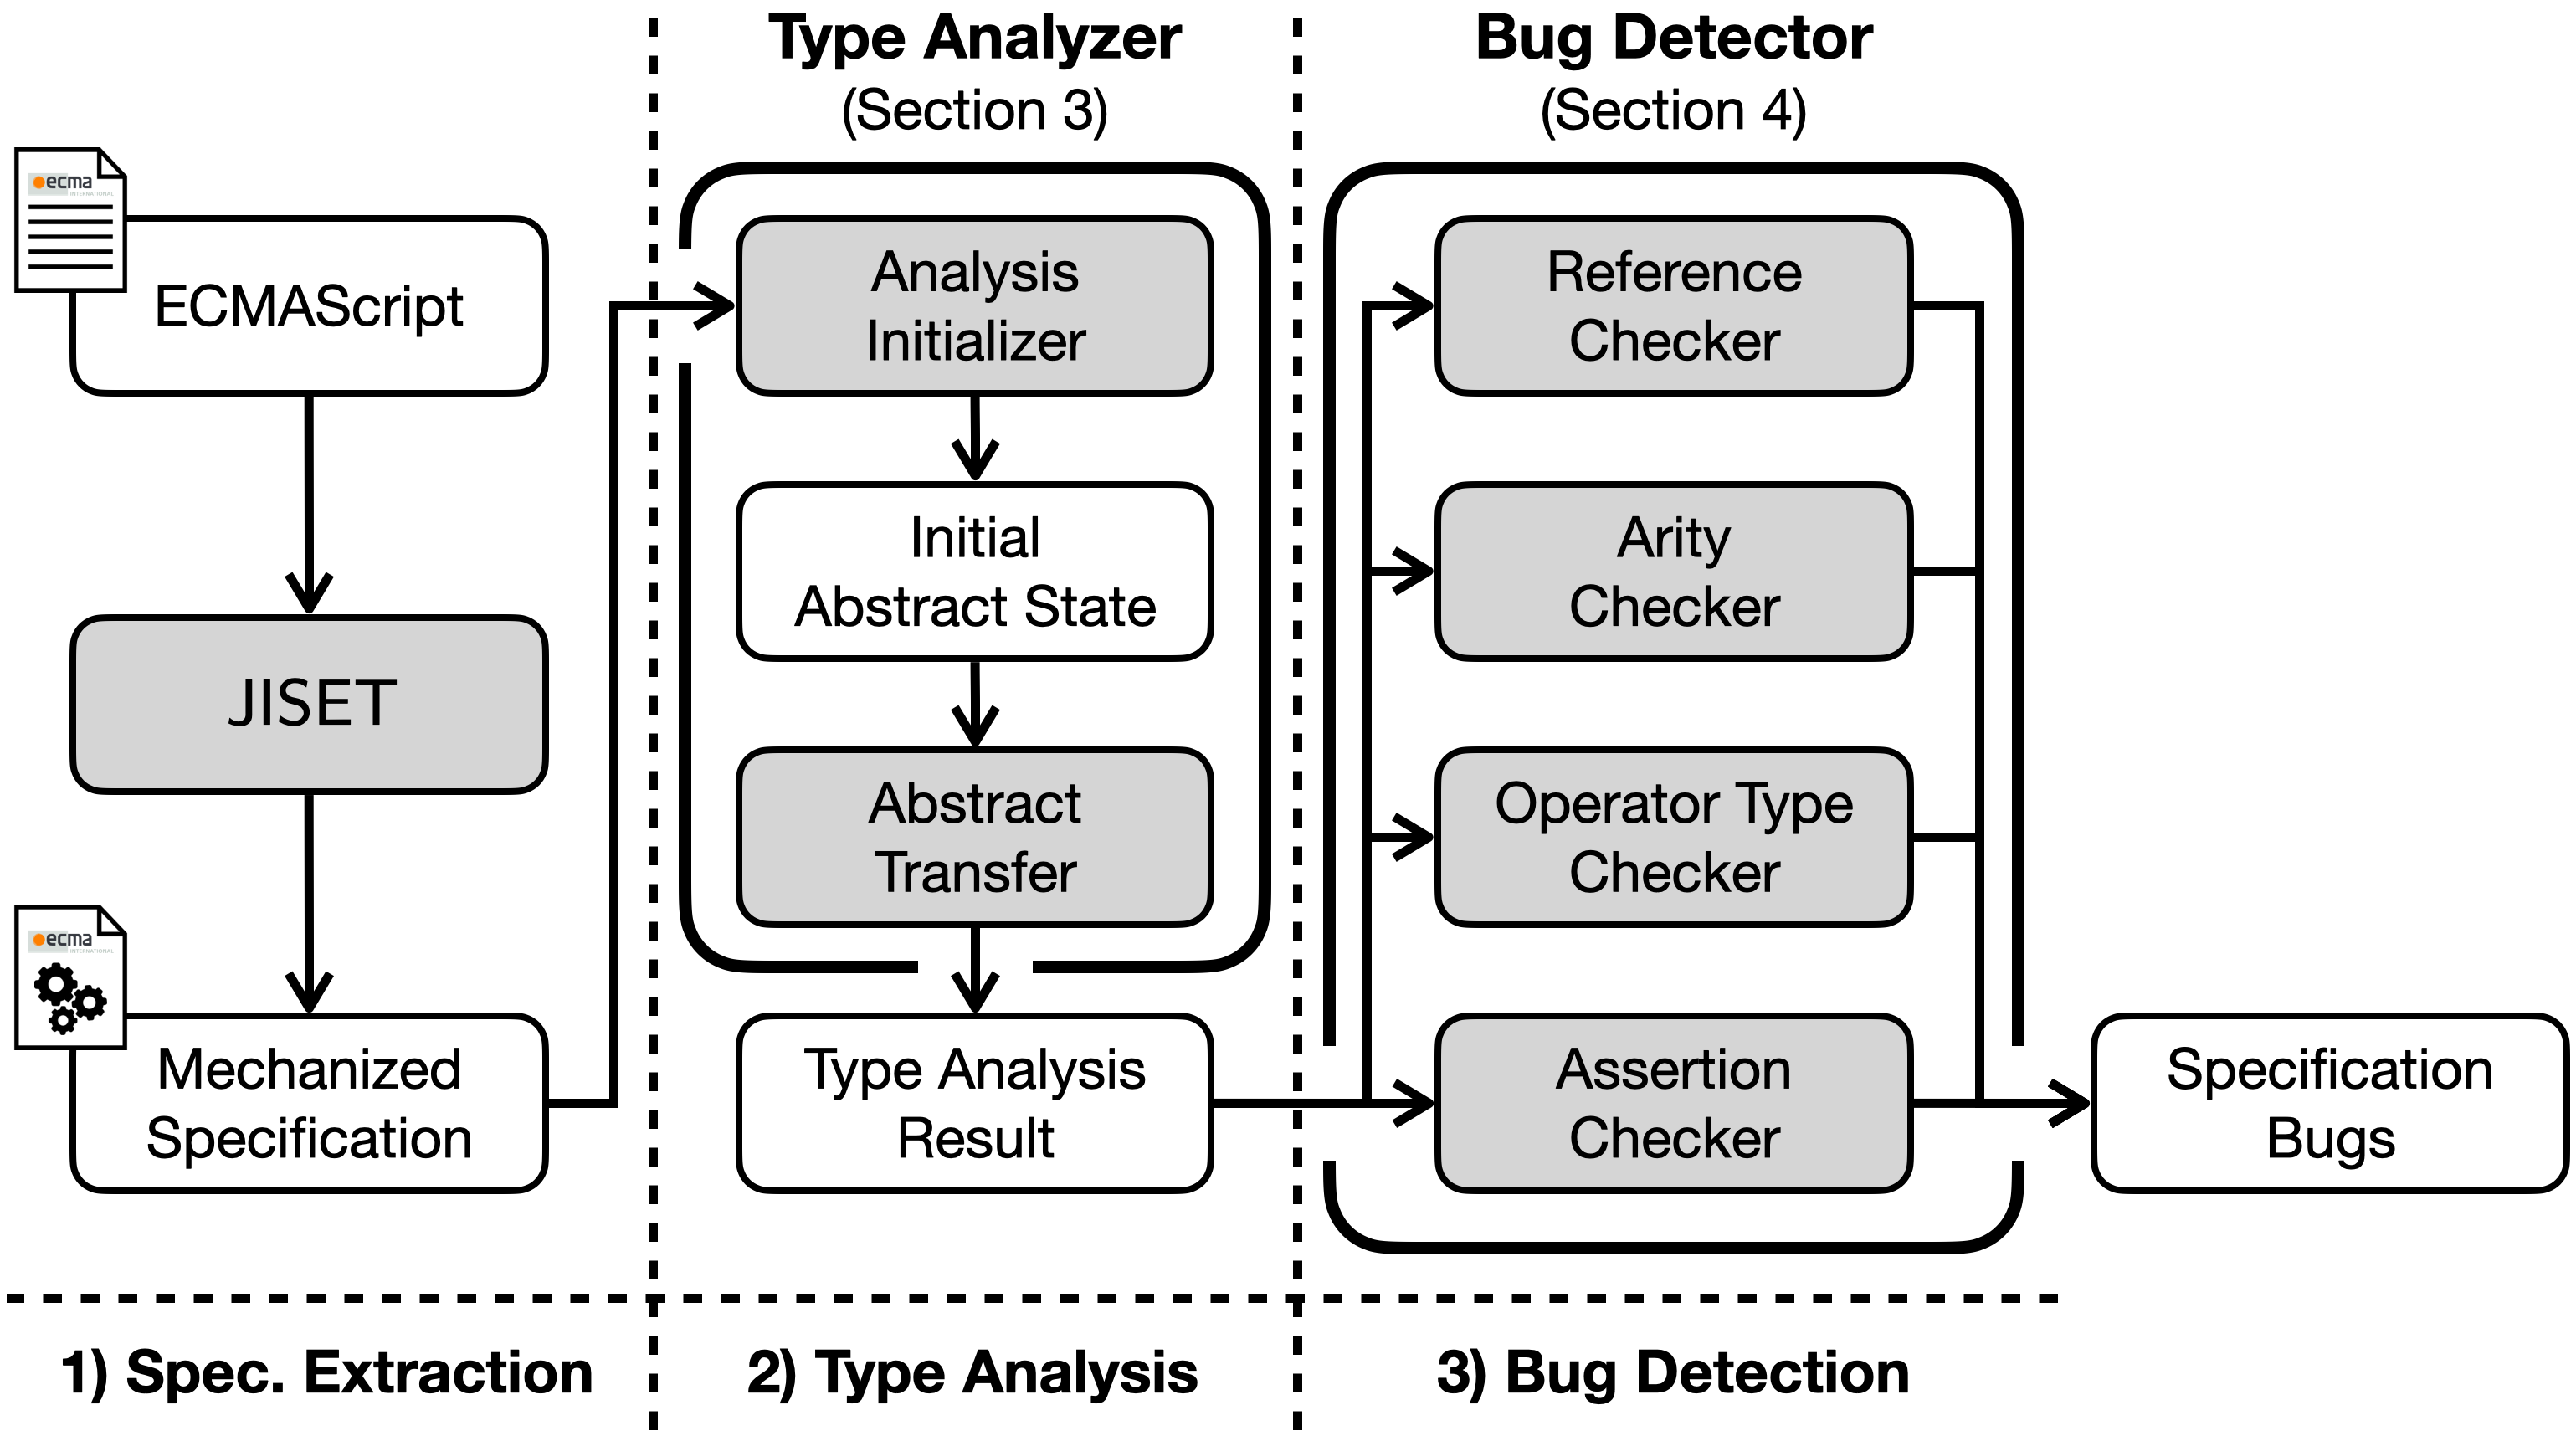
\includegraphics[width=0.48\textwidth]{img/overall}
  \vspace*{-1.5em}
  \caption{Overall structure of $\tool$: a type analyzer and a bug detector for
  mechanized specifications extracted from ECMAScript by $\jiset$.}
  \label{fig:overall}
  \vspace*{-1.5em}
\end{figure}

\begin{figure*}[t]
  \centering
  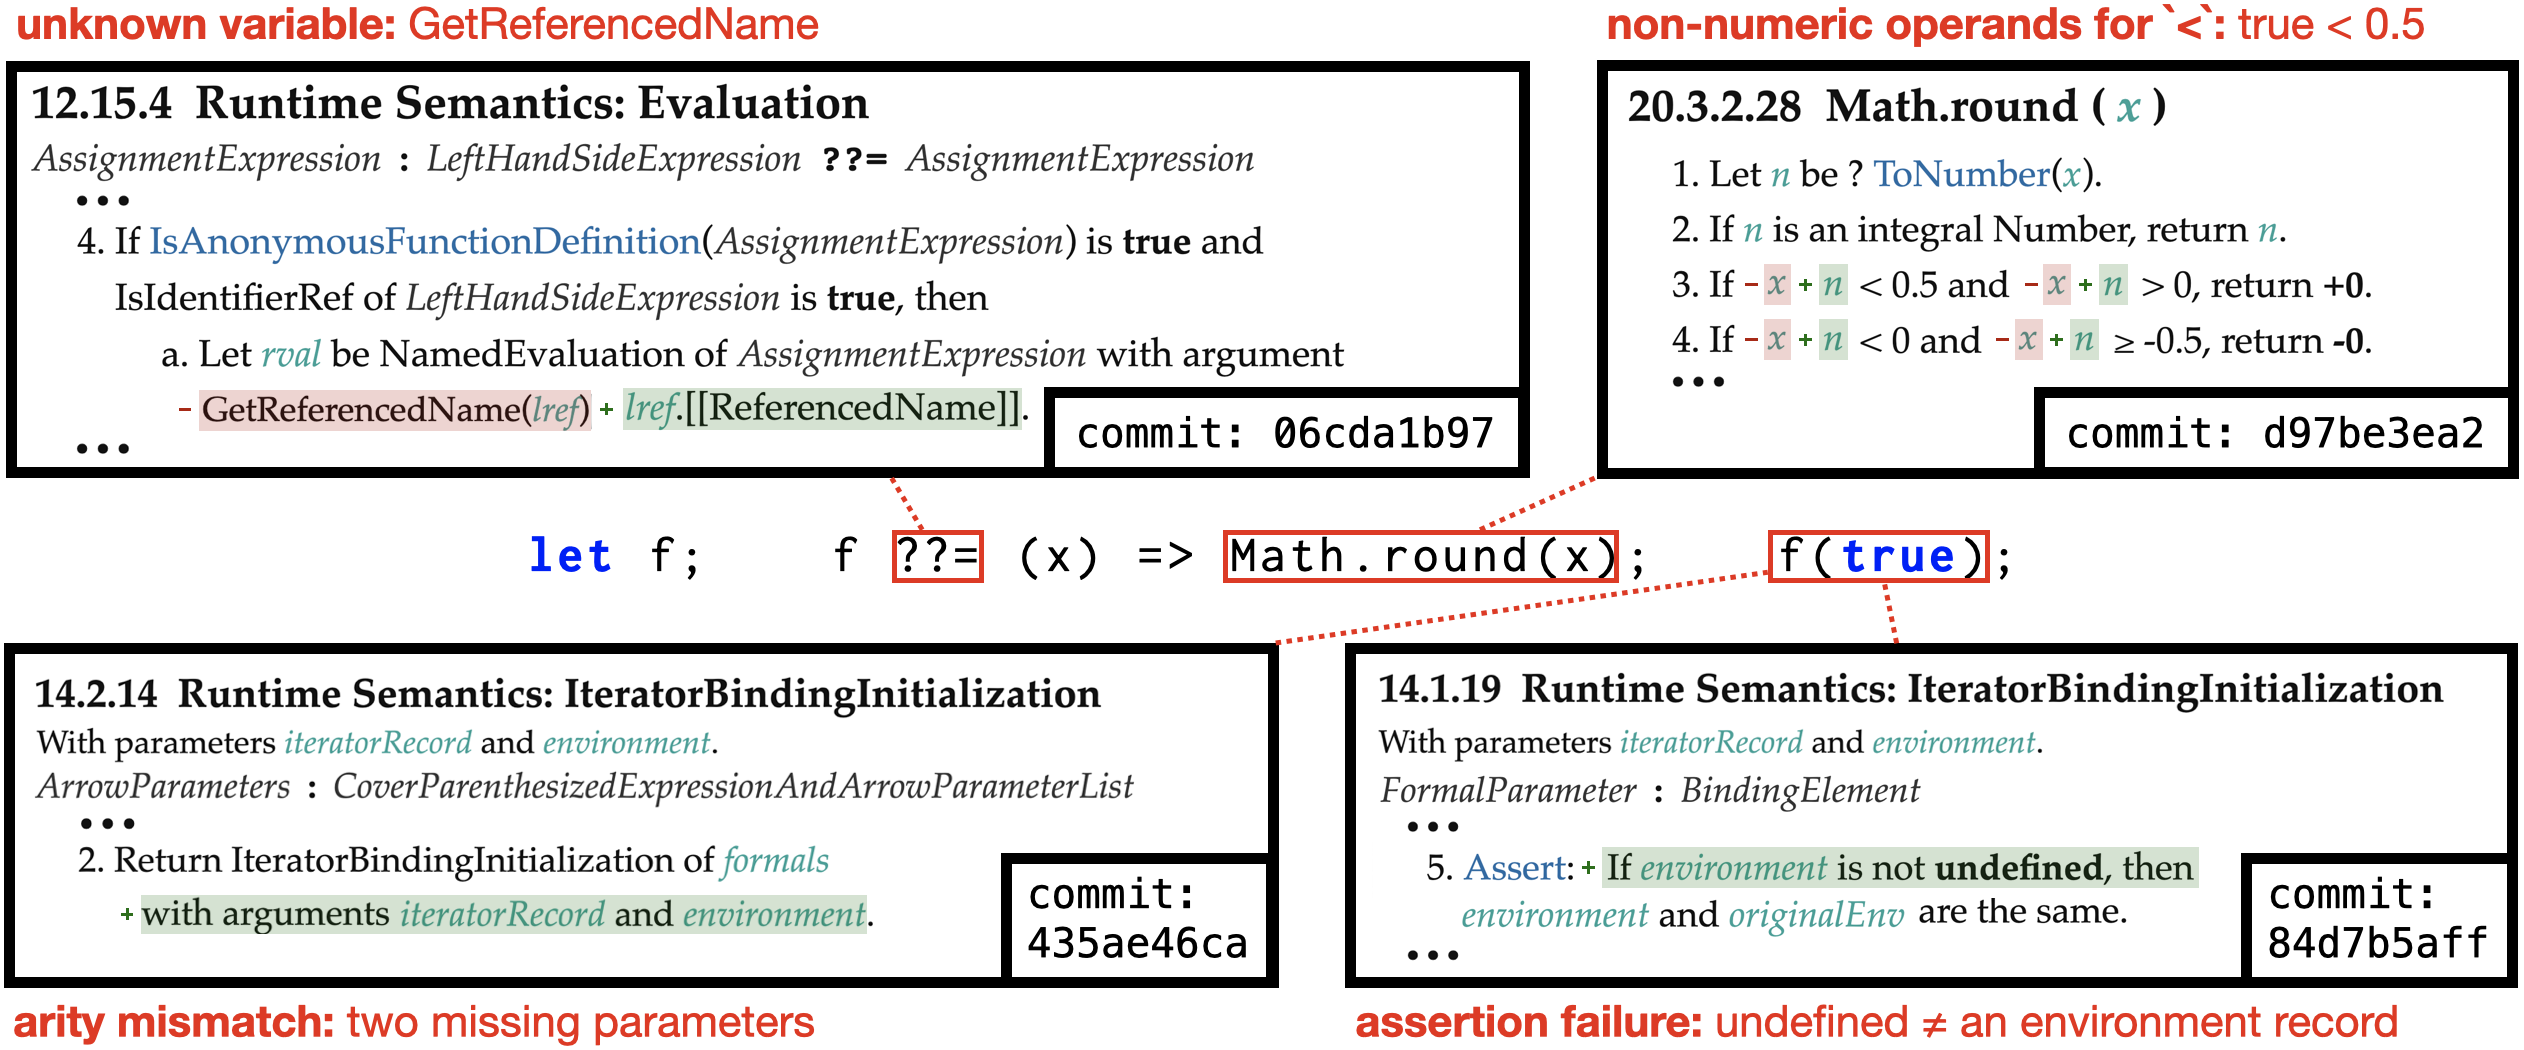
\includegraphics[width=0.9\textwidth]{img/example}
  \vspace*{-1em}
  \caption{An example JavaScript program with related previous specification
  bugs and their bugfixes.}
  \label{fig:example}
\end{figure*}
% XXX
% \begin{lstlisting}[style=FigureJS]
% let f;    f ??= (x) => Math.round(x);    f(true);
% \end{lstlisting}

In this section, we demonstrate overall structure of $\tool$ depicted in
Figure~\ref{fig:overall}.  Our tool consists of three different steps:
1) specification extraction, 2) type analysis, and 3) bug detection.


\subsection{Specification Extraction}\label{sec:overview-spec-extract}

ECMAScript describes JavaScript syntax and semantics written in a structured
natural language.  We utilize $\jiset$ to extract mechanized specification from
a given ECMAScript.

\paragraph{Syntax and Semantics} ECMAScript uses a variant of extended BNF
notations to describe JavaScript syntax.  $\jiset$ synthesizes AST structures
and JavaScript parsers from its lexical and syntactic productions.  Our tool
utilizes only AST structures to define AST types and to access corresponding
syntax-directed algorithms.  For JavaScript semantics, ECMAScript contains
abstract algorithms written in a structured natural language.  $\jiset$ compiles
them to functions of $\ires$, an untyped intermediate representation for
ECMAScript.  For brevity, we will formally define syntax and semantics of
a simplified $\ires$ in Section~\ref{sec:ires}.

\paragraph{Types} In ECMAScript, types denote not only JavaScript types but also
specification types for ASTs, internal records, and internal lists.  For ASTs,
we use non-terminal names as thier type names and AST types $A$ and $B$ have a
subtype relation $A \subtype B$ when $A$ is an alternative of $B$.  If record
types have names, we treat them as normal types and manually define their fields
according to the latest version of ECMAScript.  For example, fields of the
\code{Realm} record types are defined in ``Table 23: Realm Record Fields'' in
ECMAScript.  Ohterwise, we define structural types for unnamed record types.
For lists, we define \code{Nil} types for empty lists and parametric list types
\code{List[T]} for lists whose elements have \code{T} type.


\subsection{Type Analysis}\label{sec:overview-type-analysis}

The type analyzer performs flow-sensitive type analysis with type-sensitivity
for parameters to precisely detect specification bugs.  It consists of two
sub-modules: an \textit{analysis initializer} and an \textit{abstract transfer}.
We use a stack-based worklist algorithm to calculate fixpoint of abstract
transfer and assign the initial set of worklist using analysis initializer.

\paragraph{Analysis Initializer} In ECMAScript, there are three different kinds
of abstract algorithms \textit{normal}, \textit{syntax-directed} and
\textit{built-in}.  Since all the parameter types are known for built-in
algorithms and syntax-directed algorithms having no additional parameters, we
utilize them as entry points of type analysis.  For each entry point, the
initializer defines its abstract environment with parameter types and push the
pair of entry point and its abstract environment to the worklist.

\paragraph{Abstract Transfer} For each iteration, the abstract transfer gets a
pair of a control point and its abstract environment from the worklist, produces
other pairs based on abstract semantics, and pushes them to the worklist.  The
iteration will be finished when the worklist becomes empty.


\subsection{Bug Detection}\label{sec:overview-bug-detect}

To detect specification bugs based on the result of type analysis, we develop
four different checkers in the bug detector.  We explain targets of checkers
using an example JavaScript program with related previous specification bugs and
their bugfixes descirbed in Figure~\ref{fig:example}.

\paragraph{Reference Checker} The example JavaScript program first defines a
variable \jscode{f} without initialization thus it stores \jscode{undefined}.
Then, it assigns an arrow function to \jscode{f} using the operator
\jscode{??=}.  While the corresponding \textbf{Evaluation} algorithm originally
used \textbf{GetReferencedName} algorithm to get reference name at line 4.a, a
contributor removed the \textbf{GetReferencedName} algorithm and replaced its
all invocations to accesses of the field [[ReferencedName]] on October 28, 2020.
However, there were several missing cases including the semantics of
\jscode{??=} until another contributor fixed this bug on November 3, 2020.
Thus, an unknown variable bug of \textbf{GetReferencedName} lated for 6 days.
The reference checker detects reference bugs including unknown variable bugs.

\paragraph{Arity Checker} After the program assigns an arrow function to
\jscode{f}, it calls the function with an argument \jscode{true}.  During the
initialization of a function call, the \textbf{IteratorBindingInitialization}
algorithm is evaluated with additional parameters \textit{iteratorRecord} and
\textit{environment} to assigns arguments to proper parameters.  However, a
contributor missed the additional parameters at line 2 in the
\textbf{IteratorBindingInitialization} of \textit{ArrowParameters} on September
6, 2018.  It caused an arity mismatch bug and lasted for 532 days until another
contributor fixed this bug on February 20, 2020.  The arity checker checks such
arity mismatches.

\paragraph{Assertion Checker} During the initialization of the function call,
another specification bug existed in \textbf{IteratorBindingInitialization} of
\textit{FormalParameter}.  The additional \textit{environment} parameter might
contains \jscode{undefined} or an environment record exactly same with
\textit{originalEnv} as described in the assertion at line 5.  However, a
contributor initially added the assertion without considering of
\jscode{undefined} on \inred{XXXXXX XX, XXXX}.  Thus, the assertion failure bug
lasted for \inred{XXXX} days until April 10, 2019.  The assertion checker checks
whether such assertions are failed or not.

\paragraph{Operand Type Checker} The last checker checks whether operand types
are correct for typed operators.  After the function call initialization, the
parameter \jscode{x} points to \jscode{true} thus \jscode{Math.round} is invoked
with the argument \jscode{true}.  The \jscode{Math.round} built-in library
first converts the given parameter \textit{x} to the corresponding number value
\textit{n} using \textbf{ToNumber} algorithm, and then performs remaining steps
using the number value \textit{n}.  However, a contributor made a mistake of
using \textit{x} instead of \textit{n} at line 3 and 4 on September 11 2020.
According to this specification, the specification tries to compare a boolean
value \jscode{true} with a numeric value 0.5 or 0 in the example JavaScript
program.  Fortunately, another contributor fixed this bug after two days.  In
the bug detector, the operand type checker detects whether the operand types are
compatible with the typed operators.

In the remainder of this paper, we explain the details of how to perform type
analysis for $\ires$ functions (Section~\ref{sec:analysis}) and how to detect
type-related specification bugs using four different checkers
(Section~\ref{sec:checker}).  After we evaluate $\tool$
(Section~\ref{sec:eval}), we discuss related work (Section~\ref{sec:related}),
and conclude (Section~\ref{sec:conclusion}).
